\documentclass[hyperref, a4paper]{article}

\usepackage{geometry}
\usepackage{titling}
\usepackage{titlesec}
% No longer needed, since we will use enumitem package
% \usepackage{paralist}
\usepackage{enumitem}
\usepackage{footnote}
\usepackage{enumerate}
\usepackage{amsmath, amssymb, amsthm}
\usepackage{mathtools}
\usepackage{bbm}
\usepackage{cite}
\usepackage{graphicx}
\usepackage{subfigure}
\usepackage{physics}
\usepackage{tensor}
\usepackage{siunitx}
\usepackage[version=4]{mhchem}
\usepackage{tikz}
\usepackage{xcolor}
\usepackage{listings}
\usepackage{autobreak}
\usepackage[ruled, vlined, linesnumbered]{algorithm2e}
\usepackage{nameref,zref-xr}
\zxrsetup{toltxlabel}
\usepackage[colorlinks,unicode]{hyperref} % , linkcolor=black, anchorcolor=black, citecolor=black, urlcolor=black, filecolor=black
\usepackage[most]{tcolorbox}
\usepackage{prettyref}

% Page style
\geometry{left=3.18cm,right=3.18cm,top=2.54cm,bottom=2.54cm}
\titlespacing{\paragraph}{0pt}{1pt}{10pt}[20pt]
\setlength{\droptitle}{-5em}
\preauthor{\vspace{-10pt}\begin{center}}
\postauthor{\par\end{center}}

% More compact lists 
%\setlist[itemize]{
    %itemindent=17pt, 
    %leftmargin=1pt,
    %listparindent=\parindent,
    %parsep=0pt,
%}

% Math operators
\DeclareMathOperator{\timeorder}{\mathcal{T}}
\DeclareMathOperator{\diag}{diag}
\DeclareMathOperator{\legpoly}{P}
\DeclareMathOperator{\primevalue}{P}
\DeclareMathOperator{\sgn}{sgn}
\newcommand*{\ii}{\mathrm{i}}
\newcommand*{\ee}{\mathrm{e}}
\newcommand*{\const}{\mathrm{const}}
\newcommand*{\suchthat}{\quad \text{s.t.} \quad}
\newcommand*{\argmin}{\arg\min}
\newcommand*{\argmax}{\arg\max}
\newcommand*{\normalorder}[1]{: #1 :}
\newcommand*{\pair}[1]{\langle #1 \rangle}
\newcommand*{\fd}[1]{\mathcal{D} #1}
\DeclareMathOperator{\bigO}{\mathcal{O}}

% TikZ setting
\usetikzlibrary{arrows,shapes,positioning}
\usetikzlibrary{arrows.meta}
\usetikzlibrary{decorations.markings}
\tikzstyle arrowstyle=[scale=1]
\tikzstyle directed=[postaction={decorate,decoration={markings,
    mark=at position .5 with {\arrow[arrowstyle]{stealth}}}}]
\tikzstyle ray=[directed, thick]
\tikzstyle dot=[anchor=base,fill,circle,inner sep=1pt]

% Algorithm setting
% Julia-style code
\SetKwIF{If}{ElseIf}{Else}{if}{}{elseif}{else}{end}
\SetKwFor{For}{for}{}{end}
\SetKwFor{While}{while}{}{end}
\SetKwProg{Function}{function}{}{end}
\SetArgSty{textnormal}

\newcommand*{\concept}[1]{{\textbf{#1}}}

% Embedded codes
\lstset{basicstyle=\ttfamily,
  showstringspaces=false,
  commentstyle=\color{gray},
  keywordstyle=\color{blue}
}

% Color boxes
\tcbuselibrary{skins, breakable, theorems}
\newtcbtheorem[number within=section]{warning}{Warning}%
  {colback=orange!5,colframe=orange!65,fonttitle=\bfseries, breakable}{warn}
\newtcbtheorem[number within=section]{note}{Note}%
  {colback=green!5,colframe=green!65,fonttitle=\bfseries, breakable}{note}

\newcommand{\opticsdoc}{\href{../optics/optics}{the optics note}}
\newcommand{\soliddoc}{\href{../solid/solid}{the solid state physics note}}

\newrefformat{fig}{Figure~\ref{#1} on page~\pageref{#1}}
\newrefformat{sec}{Section~\ref{#1}}

% Support for tensor double arrows.
\renewcommand{\tensor}[1]{ \stackrel{\leftrightarrow}{\vb*{#1}}}

% Disable unsupported commands in bookmark titles 
\pdfstringdefDisableCommands{%
  \def\\{}%
  \def\texttt#1{<#1>}%
  \def\mathbb#1{#1}%
}
\pdfstringdefDisableCommands{\def\eqref#1{(\ref{#1})}}

\makeatletter
\pdfstringdefDisableCommands{\let\HyPsd@CatcodeWarning\@gobble}
\makeatother

\title{Mode-Coupling Theory of the Glass Transition}
\author{Jinyuan Wu}

\begin{document}

\maketitle

The \concept{Mode-Coupling Theory (MCT)} is the only known theory about glass transition that are
first-principles-based \cite{mct2005,mct-primer}. It uses the Mori-Zwanzig formalism 
\cite{MoriZwanzigformalismWikipedia} to integrate out unnecessary degrees of freedom and focuses 
on quantities that characterize glasses.

\section{A review of Mori-Zwanzig formalism}

First we have a brief review of the Mori-Zwanzig formalism. 
It says that any time-dependent quantity $A$ obeying the (generalized) Heisenberg equation 
\begin{equation}
    \dv*{A}{t} = \ii \mathcal{L} A
\end{equation}
also obeys the closed-form equation
\begin{equation}
    {\dot {A}}(t)= \ii \Omega A(t) - \int _{0}^{t} \dd{s} K(s)A(t-s)+F(t).
    \label{eq:closed-form-a}
\end{equation}
The three terms on the RHS are named as the \concept{frequency matrix}, the \concept{memory function}, 
and the \concept{fluctuating force}, respectively. The fluctuating force collects all ``fast'' variables that 
are orthogonal to $A$, and the memory function is the time autocorrelation function of the fluctuating force.
These two terms represent how $A$ gets connected to (in the case in a quantum theory, entangled with) the degrees of
freedom that are ignored. Generally speaking, the fluctuating force is something like the Langevin force, while 
the memory functions encodes how the system damps.  
Assuming we already have an inner product defined on physical quantities, which is usually 
\begin{equation}
    (A, B) = \expval*{A^* B},
    \label{eq:inner-product-def}
\end{equation}
The complex conjugate is motivated by the same argument in quantum field theories, i.e. if $A, B$ are Fourier 
components of real variables $\varphi, \psi$, then $\expval*{\varphi \psi}$ can be expanded into a sum of 
$\expval*{A^* B}$ terms, where $A$ and $B$ are indexed by the same frequency.
We have 
\begin{equation}
    \ii \Omega =(A, \ii \mathcal{L} A)(A,A)^{-1},
\end{equation}
\begin{equation}
    F(t)= \ee^{\ii t(1-\mathcal{P}) \mathcal{L}}\ii (1-\mathcal{P}) \mathcal{L} A
    = \ee^{\ii t(1-\mathcal{P}) \mathcal{L}} (\dot{A} - \ii \Omega A), \quad (F(t), A(0)) = 0,
\end{equation}
and 
\begin{equation}
    K(t)=- (\ii \mathcal{L} F(t),A)(A,A)^{-1} = (F(0), F(t)) (A,A)^{-1},
    \label{eq:k-def}
\end{equation}
where 
\begin{equation}
    \mathcal{P} X=(A,A)^{-1}(X,A)A.
\end{equation}
Note that the convention of notation varies in the literature, and the two expressions of $K(t)$ in \eqref{eq:k-def}
can both be seen. We require $A$ to be ``slow'' variables (or satisfy other conditions that somehow separate it 
from other degrees of freedom), or otherwise fluctuation is too strong for $A$ to be a useful quantity.

Of course we can have several slow variables and several fast variables. Therefore, we may replace $A$ by a vector. 
Note that at this time, $\Omega, F$ and $K$ are matrices, and it can be found that \eqref{eq:inner-product-def}
should be replaced by 
\begin{equation}
    \expval*{A, B} = \expval*{A^* B^\top},
\end{equation} 
instead of 
\[
    \expval*{A, B} = \expval*{A^\dagger B}.
\]

\section{Motivation of MCT}

\begin{figure}
    \centering
    

\tikzset{every picture/.style={line width=0.75pt}} %set default line width to 0.75pt        

\begin{tikzpicture}[x=0.75pt,y=0.75pt,yscale=-1,xscale=1]
%uncomment if require: \path (0,378); %set diagram left start at 0, and has height of 378

%Straight Lines [id:da2866989210872881] 
\draw    (92,242) -- (576,242) ;
\draw [shift={(578,242)}, rotate = 180] [fill={rgb, 255:red, 0; green, 0; blue, 0 }  ][line width=0.08]  [draw opacity=0] (12,-3) -- (0,0) -- (12,3) -- cycle    ;
%Straight Lines [id:da4373164359721642] 
\draw    (194,242) ;
\draw [shift={(194,242)}, rotate = 0] [color={rgb, 255:red, 0; green, 0; blue, 0 }  ][fill={rgb, 255:red, 0; green, 0; blue, 0 }  ][line width=0.75]      (0, 0) circle [x radius= 3.35, y radius= 3.35]   ;
%Straight Lines [id:da9393368773961788] 
\draw    (217,242) ;
\draw [shift={(217,242)}, rotate = 0] [color={rgb, 255:red, 0; green, 0; blue, 0 }  ][fill={rgb, 255:red, 0; green, 0; blue, 0 }  ][line width=0.75]      (0, 0) circle [x radius= 3.35, y radius= 3.35]   ;
%Straight Lines [id:da5363038804777169] 
\draw    (530,242) ;
\draw [shift={(530,242)}, rotate = 0] [color={rgb, 255:red, 0; green, 0; blue, 0 }  ][fill={rgb, 255:red, 0; green, 0; blue, 0 }  ][line width=0.75]      (0, 0) circle [x radius= 3.35, y radius= 3.35]   ;
%Straight Lines [id:da22573584972311234] 
\draw    (378,242) ;
\draw [shift={(378,242)}, rotate = 0] [color={rgb, 255:red, 0; green, 0; blue, 0 }  ][fill={rgb, 255:red, 0; green, 0; blue, 0 }  ][line width=0.75]      (0, 0) circle [x radius= 3.35, y radius= 3.35]   ;
%Straight Lines [id:da8217101511374114] 
\draw    (399,242) ;
\draw [shift={(399,242)}, rotate = 0] [color={rgb, 255:red, 0; green, 0; blue, 0 }  ][fill={rgb, 255:red, 0; green, 0; blue, 0 }  ][line width=0.75]      (0, 0) circle [x radius= 3.35, y radius= 3.35]   ;

% Text Node
\draw (580,242) node [anchor=west] [inner sep=0.75pt]    {$T$};
% Text Node
\draw (194,247.4) node [anchor=north] [inner sep=0.75pt]    {$T_{\text{0}}$};
% Text Node
\draw (121,233) node [anchor=south west] [inner sep=0.75pt]   [align=left] {entropy crisis: no liquid \\is possible below $\displaystyle T_{\text{K}}$};
% Text Node
\draw (530,247.4) node [anchor=north] [inner sep=0.75pt]    {$T_{\text{m}}$};
% Text Node
\draw (479,335) node [anchor=south west] [inner sep=0.75pt]   [align=left] {melting point; \\supercooled \\liquid below $\displaystyle T_{\text{m}}$};
% Text Node
\draw (217,247.4) node [anchor=north] [inner sep=0.75pt]    {$T_{\text{K}}$};
% Text Node
\draw (116,311) node [anchor=south west] [inner sep=0.75pt]   [align=left] {infinite viscosity: no \\equilibrium below $\displaystyle T_{0}$};
% Text Node
\draw (378,247.4) node [anchor=north] [inner sep=0.75pt]    {$T_{\text{g}}$};
% Text Node
\draw (399,247.4) node [anchor=north] [inner sep=0.75pt]    {$T_{\text{c}}$};
% Text Node
\draw (312,192) node [anchor=north west][inner sep=0.75pt]   [align=left] {Naive MCT predicts non- \\ergodic behavior below $\displaystyle T_{\text{c}}$};
% Text Node
\draw (315,272) node [anchor=north west][inner sep=0.75pt]   [align=left] {$\displaystyle T_{\text{g}}$: experimental\\transition temperature;\\position uncertain};


\end{tikzpicture}

    \caption{Important temperature points. As the temperature goes down, first the liquid becomes overcooled,
    and if the liquid is fragile, two-step relaxation occurs. The $T_\text{c}$ is a dynamic phase transition }
\end{figure}

Now we go back to derive a theory about glass transition. \concept{Mode coupling theory} is a so-called 
\emph{generalized} hydrodynamic theory for glasses \cite{RevModPhys.76.785,Cummins_1999} in that it 
still only considers density fluctuations in the system, but the density fluctuations are not smoothened. 
We will find a closed equation about the density-density correlation function, and observe its time evolution.

Here we consider some motivation of MCT. We already know that glasses are like liquids in that there is no 
broken spacial translational symmetry, but glasses are not just (simple) liquids in that there are some 
weird things happening. That is the reason we need a \emph{hydrodynamic} theory which focuses on density 
modes, which can be measured directly using scattering experiments \cite{mct2005}, but the theory must
be more than ordinary Navier-Stokes equations to include microscopic details. We know glass transition is 
of kinetic nature, and therefore a quantitative theory of it must be a dynamic one. A hydrodynamic theory 
is a dynamic theory, but it does not capture essential microscopic details of a supercooled liquid and 
therefore cannot explain glass transition. A microscopic thermodynamic theory (or a theory invoking thermodynamic 
concepts to explain the dynamic behavior of a system, for example the Adam-Gibbs theory \cite{Sengupta_2012})
captures the microscopic details relevant in glass transition, but is unable to capture some dynamic details
like two-step relaxation. We hope a generalized hydrodynamic theory can mix the advantages of the two 
approaches together.

Note that the spacial translation symmetry gives 
\begin{equation}
    \expval*{\rho(0, 0) \rho(\vb*{r}, t)} = \frac{1}{V} \int \frac{\dd[3]{\vb*{k}}}{(2\pi)^3} 
    \ee^{- \ii \vb*{k} \cdot \vb*{r}} \expval*{\rho_{-\vb*{k}}(0) \rho_{\vb*{k}}(t)},
\end{equation}
and since no valuable information is provided when $\abs*{\vb*{r}} \to 0$, we will work on the correlation function
in the momentum space to separate different spatial scales.
What we are going to do is to find a self-consistent equation about the density-density correlation function in 
the small momentum region (or the large $\abs*{\vb*{r}}$ region). We denote the correlation function as 
\begin{equation}
    F(k, t)=\frac{1}{N}\left\langle\rho_{-\vb*{k}}(0) \rho_{\vb*{k}}(t)\right\rangle=\frac{1}{N} \sum_{i j}\left\langle \ee^{-\ii \vb*{k} \cdot \vb*{r}_{i}(0)} \ee^{\ii \vb*{k} \cdot \vb*{r}_{j}(t)}\right\rangle,
\end{equation}
where 
\begin{equation}
    \begin{aligned}
        \rho_{\vb*{k}}(t) &= \int \dd[3]{\vb*{r}} \ee^{\ii \vb*{k} \cdot \vb*{r}} \rho(\vb*{r}, t) \\
        &=\sum_{i} \int \dd[3]{\vb*{r}} \ee^{\ii \vb*{k} \cdot \vb*{r}} \delta\left(\vb*{r}-\vb*{r}_{i}(t)\right) \\
        &=\sum_{i} \ee^{\ii \vb*{k} \cdot \vb*{r}_{i}(t)}.
    \end{aligned}
\end{equation}
Specifically, we have 
\begin{equation}
    F(k, 0) = S(k),
\end{equation}
which is the static structural factor.

\begin{note*}{}{}
    If we are discussing a quantum system, we need to be more clear here about whether the density modes we are
    talking about are operators or expectations. If we are talking about a theory of density operators, 
    this is known as (a hydrodynamic flavor of) bosonization. If we are talking about a theory of expectation
    of density operators, this is known as (hydrodynamic approach) of kinetic theory or (dynamic) density 
    functional theory. All these approaches are different in a quantum many-body theory context, but 
    since we are talking about a system where quantum fluctuation is not important, we can consider these 
    approaches being equivalent, and call them \emph{hydrodynamic} or \emph{generalized hydrodynamic} ones. 
\end{note*}

\section{The exact time-evolution equation of the correlation function} 

The derivation shown below is mainly based on \cite{mct2005}, but the notation is from \cite{RevModPhys.76.785}. 

We are going to apply the Mori-Zwanzig formalism to $F(k, t)$. We need to find some slow variables
and apply \eqref{eq:closed-form-a} to them to find their dynamics, and then we are able to find the dynamics 
of $F(k, t)$. It can be easily noticed that since we are interested in the small $k$ region, the time derivative 
\[
    \dot{\rho}_{\vb*{k}} = \sum_i \frac{\ii \vb*{k} \cdot \vb*{p}_i}{m} \ee^{\ii \vb*{k} \cdot \vb*{r}_i }
\]
is also small, and therefore $\rho_{\vb*{k}}(t)$ is a slow variable. Then we also find that 
\[
    \ii \abs*{\vb*{k}} j_{\vb*{k}}^\text{L} = \ii \vb*{k} \cdot 
    \underbrace{\sum_{i} \frac{\vb*{p}_i}{m} \ee^{\ii \vb*{k} \cdot \vb*{r}}}_{\vb*{j}_{\vb*{k}}}
\]
is a slow variable. So the slow variable set is 
\begin{equation}
    \vb{A} = \pmqty{\var{\rho_{\vb*{k}}} \\ j_{\vb*{k}}^\text{L}},  
\end{equation}
where 
\begin{equation}
    \var{\rho_{\vb*{k}}} = \rho_{\vb*{k}} - \expval*{\rho_{\vb*{k}}} 
    = \sum_{i} \ee^{\ii \vb*{q} \cdot \vb*{r}_i} - (2\pi)^3 \rho \delta(\vb*{q}).
\end{equation}

Applying \eqref{eq:closed-form-a} to $\vb{A}$, we have 
\[
    \dot{\vb{A}}(t)= \ii \vb{\Omega} \vb{A}(t) - \int_{0}^{t} \dd{s} \vb{K}(s) \vb{A}(t-s)+ \vb{F}(t),
\]
and since 
\[
    \expval*{\vb{A}(0), \vb{F}(t)} = \expval*{\vb{A}(0)^* \vb{F}(t)^\top} = 0, 
\]
which is a result in the Mori-Zwanzig formalism, we have 
\begin{equation}
    \dot{\vb{C}} = \ii \vb{\Omega} \vb{C}(t) - \int_{0}^{t} \dd{s} \vb{K}(s) \vb{C}(t-s),
    \label{eq:matrix-eq}
\end{equation}
where we have 
\begin{equation}
    \vb{C}(t) = \expval*{\vb{A}(0)^* \vb{A}(t)^\top} = \pmqty{\left\langle\delta \rho_{-\vb*{q}}(0) \delta \rho_{\vb*{q}}(t)\right\rangle & \left\langle\delta \rho_{-\vb*{q}}(0) j_{\vb*{q}}^\text{L}(t)\right\rangle \\
    \left\langle - j_{-\vb*{q}}^\text{L}(0) \delta \rho_{\vb*{q}}(t)\right\rangle & \left\langle - j_{-\vb*{q}}^\text{L}(0) j_{\vb*{q}}^\text{L}(t)\right\rangle},
    \label{eq:c-eq}
\end{equation}
\begin{equation}
    \begin{aligned}
        \ii \vb{\Omega} &= \expval*{\vb{A}, \dot{\vb{A}}} \expval*{\vb{A}, \vb{A}}^{-1} \\
        &= \pmqty{ 
            \expval*{\var{\rho_{-\vb*{q}}} \var{\dot{\rho}_{\vb*{q}}} } &
            \expval*{\var{\rho_{-\vb*{q}}} \var{\dot{j}^\text{L}_{\vb*{q}}} } \\
            \expval*{-\var{j^\text{L}_{-\vb*{q}}} \var{\dot{\rho}_{\vb*{q}}} } &
            \expval*{-\var{j^\text{L}_{-\vb*{q}}} \var{\dot{j}^\text{L}_{\vb*{q}}} }} 
        \pmqty{ 
            \expval*{\var{\rho_{-\vb*{q}}} \var{{\rho}_{\vb*{q}}} } &
            \expval*{\var{\rho_{-\vb*{q}}} \var{{j}^\text{L}_{\vb*{q}}} } \\
            \expval*{-\var{j^\text{L}_{-\vb*{q}}} \var{{\rho}_{\vb*{q}}} } &
            \expval*{-\var{j^\text{L}_{-\vb*{q}}} \var{{j}^\text{L}_{\vb*{q}}} } }^{-1}
    \end{aligned}
    \label{eq:omega-def}
\end{equation}
Note that unitarity guarantees that the $\expval*{\vb{A}, \vb{A}}$ factor in \eqref{eq:omega-def} is constant,
and therefore we have 
\begin{equation}
    \expval*{\vb{A}, \vb{A}} = \pmqty{ 
            \expval*{\var{\rho_{-\vb*{q}}} \var{{\rho}_{\vb*{q}}} } &
            \expval*{\var{\rho_{-\vb*{q}}} \var{{j}^\text{L}_{\vb*{q}}} } \\
            \expval*{\var{j^\text{L}_{-\vb*{q}}} \var{{\rho}_{\vb*{q}}} } &
            \expval*{\var{j^\text{L}_{-\vb*{q}}} \var{{j}^\text{L}_{\vb*{q}}} } 
        } = \pmqty{
            N S(q) & 0 \\ 
            0 &  \frac{N k_\text{B} T}{m}
        },
    \label{eq:normalize}
\end{equation}
where 
\[
    \expval*{\var{\rho_{-\vb*{q}}} \var{{j}^\text{L}_{\vb*{q}}} } \propto \vb*{q} \cdot \expval*{\vb*{p}}  = 0,
\]
and 
\[
    \begin{aligned}
        \expval*{- j^\text{L}_{-\vb*{q}} j^\text{L}_{\vb*{q}}} &= 
        \sum_{i, j} \expval*{(\vu*{q} \cdot \vb*{v}_i) (\vu*{q} \cdot \vb*{v}_j)} \ee^{\ii \vb*{q} \cdot (\vb*{r}_j - \vb*{r}_i)} \\
        &= \sum_{i, j} \delta_{ij} \vb*{q} \cdot \frac{k_\text{B} T}{m}  \cdot  \vb*{q} \ee^{\ii \vb*{q} \cdot (\vb*{r}_j - \vb*{r}_i)} \\
        &= \frac{N k_\text{B} T}{m}.
    \end{aligned}
\]
Here and below we calculate all expectations with the assumption that the translational symmetry is not broken,
and therefore the probabilistic distributions of positions and momenta are independent. We also invoke the
equipartition theorem. We also should keep in mind the fact that velocities at one time step may be correlated to
the past configuration, and therefore \emph{non}-equal time correlation functions $\expval*{\rho_{-\vb*{q}}(0) j^\text{L}_{\vb*{q}}(t)}$ is not necessarily 
zero (or otherwise some weird facts will occur, like a variable is constant but its time derivative is not, etc.).
We can also evaluate the $\expval*{\vb{A}, \dot{\vb{A}}}$ factor. A variable is always 
orthogonal to its time derivative, and we have 
\[
    \expval*{\var{\rho_{-\vb*{q}}} \var{\dot{\rho}_{\vb*{q}}} } = \expval*{\var{\rho_{\vb*{q}}}, \var{\dot{\rho}_{\vb*{q}}} } = 0, \quad 
    \expval*{-\var{j^\text{L}_{-\vb*{q}}} \var{\dot{j}^\text{L}_{\vb*{q}}} } = 0,
\]
and 
\[
    \begin{aligned}
        \expval*{\var{\rho_{\vb*{q}}} \dot{j}^\text{L}_{\vb*{q}}} &= 
        \sum_i (\expval*{\var{\rho_{-\vb*{q}}} \vu*{q} \cdot \dot{\vb*{v}}_i \ee^{\ii \vb*{q} \cdot \vb*{r}_i}} +
        \underbrace{\expval*{\var{\rho_{-\vb*{q}}} \cdot \ii \vb*{q} \cdot \vb*{v}_i \ee^{\ii \vb*{q} \cdot \vb*{r}_i}}}_{\propto \expval*{\vb*{v}_i} = 0} ) \\
        &= \sum_i \expval*{\var{\rho_{-\vb*{q}}} \vu*{q} \cdot \dot{\vb*{v}}_i \ee^{\ii \vb*{q} \cdot \vb*{r}_i}} \\
        &= \sum_{i, j} \expval*{\ee^{- \ii \vb*{q} \cdot \vb*{r}_j} \var{\rho_{-\vb*{q}}} \vu*{q} \cdot \dot{\vb*{v}}_i \ee^{\ii \vb*{q} \cdot \vb*{r}_i}} \\
        &= \dv{t} \sum_{i, j} \underbrace{\expval*{\ee^{- \ii \vb*{q} \cdot \vb*{r}_j} \var{\rho_{-\vb*{q}}} \vu*{q} \cdot {\vb*{v}}_i \ee^{\ii \vb*{q} \cdot \vb*{r}_i}}}_{\propto \expval*{\vb*{v}_i} = 0} - \sum_{i, j} \expval*{ - \ii \vb*{q} \cdot \vb*{v}_j \ee^{- \ii \vb*{q} \cdot \vb*{r}_j} \var{\rho_{-\vb*{q}}} \vu*{q} \cdot {\vb*{v}}_i \ee^{\ii \vb*{q} \cdot \vb*{r}_i}} \\
        &= \ii \sum_{i, j} \expval*{ \vb*{q} \cdot \vb*{v}_j \ee^{- \ii \vb*{q} \cdot \vb*{r}_j} \var{\rho_{-\vb*{q}}} \vu*{q} \cdot {\vb*{v}}_i \ee^{\ii \vb*{q} \cdot \vb*{r}_i}} \\
        &= \ii \sum_{i, j}  \vb*{q} \cdot \frac{k_\text{B} T}{m} \tensor{\vb*{I}} \cdot \vu*{q} \ee^{\ii \vb*{q} (\vb*{r}_i - \vb*{r}_j)} \\
        &= \frac{\ii q N k_\text{B} T}{m},
    \end{aligned}
\]
and the same derivation works for $\expval*{-\var{j^\text{L}_{-\vb*{q}}} \var{\dot{\rho}_{\vb*{q}}} }$.
Therefore, \eqref{eq:omega-def} evaluates to be 
\begin{equation}
    \ii \vb{\Omega} = \pmqty{0 & \frac{\ii q N k_\text{B} T}{m} \\ \frac{\ii q N k_\text{B} T}{m} & 0} \pmqty{\dmat{NS(q), \frac{N k_\text{B} T}{m}}}^{-1} = \pmqty{0 & \ii q \\ \frac{\ii q k_\text{B} T}{m S(q)} & 0}.
    \label{eq:omega-eq}
\end{equation}
Then we need the memory matrix, which in turn requires us to find the fluctuation force. Note that if we 
are able to evaluate $\vb{F}(0)$ into a linear function of $\vb{A}(0)$, then we have already obtained 
$\vb{F}(t)$ by replacing $\vb{A}(0)$ with $\vb{A}(t)$. We have 
\[
    \vb{F}(0) = \dot{\vb{A}} - \ii \vb{\Omega} \vb{A} = \pmqty{\var{\dot{\rho}_{\vb*{q}}} \\ \dot{j}_{\vb*{q}}^\text{L}} - \pmqty{0 & \ii q \\ \frac{\ii q k_\text{B} T}{m S(q)} & 0} \pmqty{\var{\rho_{\vb*{q}}} \\ j_{\vb*{q}}^\text{L}} = \eval{\pmqty{0 \\ \dot{j}_{\vb*{q}}^\text{L} - \frac{\ii q k_\text{B} T}{m S(q)} \var{\rho}_{\vb*{q}} } }_{t=0} \eqqcolon \pmqty{0 \\ R_{\vb*{q}}(0)}, 
\]
and hence we have 
\begin{equation}
    \vb{F}(t) = \pmqty{0 \\ \dot{j}_{\vb*{q}}^\text{L} - \frac{\ii q k_\text{B} T}{m S(q)} \var{\rho}_{\vb*{q}} }
    = \pmqty{0 \\ R_{\vb*{q}}}.
    \label{eq:f-q-eq}
\end{equation}
Now the memory matrix can be obtained straightforwardly:
\begin{equation}
    \begin{aligned}
        \vb{K}(t) &= \expval{\vb{F}(0)^* \vb{F}(t)^\top} \expval*{\vb{A}, \vb{A}}^{-1} = \pmqty{0 & 0 \\ 0 & \expval*{R_{-\vb*{q}}(0) R_{\vb*{q}}(t)}} \pmqty{
        N S(q) & 0 \\ 
        0 &  \frac{N k_\text{B} T}{m}
    }^{-1} \\
    &=  \pmqty{0 & 0 \\ 0 & \frac{m}{N k_\text{B} T} \expval*{R_{-\vb*{q}}(0) R_{\vb*{q}}(t)}}.
    \end{aligned}
    \label{eq:k-eq}
\end{equation}

Now \eqref{eq:matrix-eq}, \eqref{eq:c-eq}, \eqref{eq:omega-eq}, \eqref{eq:k-eq} and the definition of $R_{\vb*{q}}$ 
in \eqref{eq:f-q-eq} form a closed group of equations. Actually we are only interested in $F(q, t)$,
and we can focus on the left bottom element of \eqref{eq:matrix-eq}, which is 
\begin{equation}
    \begin{aligned}
        \dv{t} \expval*{ - j^\text{L}_{-\vb*{q}}(0) \var{\rho}_{\vb*{q}}(t) } 
        &= \frac{\ii q k_\text{B} T}{m S(q)} \expval*{ \var{\rho}_{-\vb*{q}}(0) \var{\rho}_{\vb*{q}}(t) } \\
        &\quad - \int_0^t \dd{\tau} \frac{m}{N k_\text{B} T} \expval*{R_{-\vb*{q}}(0) R_{\vb*{q}}(\tau)} \expval*{ - j^\text{L}_{-\vb*{q}}(0) \var{\rho}_{\vb*{q}}(t - \tau) } .
    \end{aligned}
    \label{eq:original-mct}
\end{equation}
Note that the time translation symmetry guarantees
\[
    \expval*{\var{\rho_{-\vb*{q}}(-t)} \var{\rho_{\vb*{q}}(0)}} = \expval*{\var{\rho_{-\vb*{q}}(0)} \var{\rho_{\vb*{q}}(t)}},
\]
and by taking time derivative we have 
\[
    \begin{aligned}
        \dv{t} \expval*{\var{\rho_{-\vb*{q}}(0)} \var{\rho_{\vb*{q}}(t)}} &= 
        \dv{t} \expval*{\var{\rho_{-\vb*{q}}(-t)} \var{\rho_{\vb*{q}}(0)}} \\
        &= \dv{t} \sum_i \expval*{\ee^{- \ii \vb*{q} \cdot \vb*{r}_i (-t)} \var{\rho_{\vb*{q}}(0)}}  \\
        &= \sum_i \expval*{ - \ii \vb*{q} \cdot (- \vb*{v}_i(-t)) \ee^{- \ii \vb*{q} \cdot \vb*{r}_i (-t)} \var{\rho_{\vb*{q}}(0)}}  \\
        &= \ii q \expval*{- j^\text{L}_{-\vb*{q}}(-t) \var{\rho_{\vb*{q}}(0)}} \\
        &= \ii q \expval*{- j^\text{L}_{-\vb*{q}}(0) \var{\rho_{\vb*{q}}(t)}},
    \end{aligned}
\]
which means 
\[
    \begin{aligned}
        \expval*{- j^\text{L}_{-\vb*{q}}(0) \var{\rho_{\vb*{q}}(t)}} 
        &= \frac{1}{\ii q} \dv{t} \expval*{\var{\rho_{-\vb*{q}}(0)} \var{\rho_{\vb*{q}}(t)}} \\
        &= \frac{N}{\ii q} \dv{F(q, t)}{t} .
    \end{aligned}
\]
Substitution of the above equation into \eqref{eq:original-mct}, we get 
\begin{equation}
    \dv[2]{F(q, t)}{t} + \frac{q^2 k_\text{B} T}{m S(q)} F(q, t) + \frac{m}{N k_\text{B} T} \int_0^t \dd{\tau} \expval*{R_{-\vb*{q}}(0) R_{\vb*{q}}(\tau)} \dv{F(q, t)}{t} = 0,
    \label{eq:exact-mct}
\end{equation}
where 
\begin{equation}
    R_{\vb*{q}} = \dot{j}_{\vb*{q}}^\text{L} - \frac{\ii q k_\text{B} T}{m S(q)} \var{\rho}_{\vb*{q}}.
    \label{eq:r-def}
\end{equation}

\eqref{eq:exact-mct} is exact under the conditions that at least the supercooled liquid is locally in thermal
equilibrium, so we have a definition of temperature, that equipartition theorem works for the momenta 
and that spacial and temporal translational symmetries are not broken, which is obviously correct for glass. 
However, \eqref{eq:exact-mct} is \emph{not} closed in that $R_{\vb*{q}}$ should be evaluated using $\rho_{\vb*{q}}$
and $j^\text{L}_{\vb*{q}}$ instead of $\expval*{\var{\rho_{-\vb*{q}}(0)} \var{\rho_{\vb*{q}}(t)}}$. 
Therefore, we need to derive an explicit expression of $R_{\vb*{q}}$ using $F(q, t)$. 
If such an expression is not available, then we are unable to reach a generalized hydrodynamic theory 
of glass. 

\section{Closing \eqref{eq:exact-mct} and the MCT approximation}

Now we need some intuition to have an approximation of $\expval*{R_{-\vb*{q}}(0) R_{\vb*{q}}(\tau)}$.
The approximation made in this section results in a closed equation system, which is usually called 
the (simple) MCT for the memory function couples $F(q, t)$ at different momenta.

We can see the derivation above has some mean-field theoretical flavor (It even invokes the Wick theorem!). 
It can be seen as a mean-field theory of something like a replica theory \cite{Franz_2012}. To be exact,
MCT is not a typical mean-field theory, either, because it fails with infinite dimensions \cite{mct-mft-2010}.

\section{MCT's solution, its success and its failure}

Now we review what can and cannot be captured with MCT. 

\begin{figure}
    \centering
    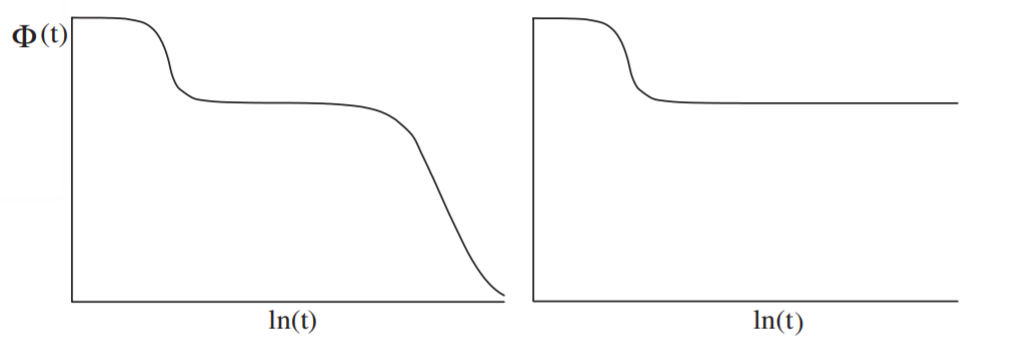
\includegraphics[width=0.9\textwidth]{glass-fig-5.PNG}
    \caption{Figure~5 from \cite{mct2005}.}
\end{figure}

The largest problem is probably that MCT predicts that there is almost a dynamic phase transition%
\footnote{Dynamic phase transition does happen from time to time in non-equilibrium systems. 
See \cite{Heyl_2019}, for example.}
at $T = T_\text{c}$ \cite{2004-critical}, with divergent viscosity and a clear ergodic-non-ergodic distinction. 
We already know this is not the case. First, we already know that $T_\text{g}$ is dependent to the time scale 
of the observation. Some may argue that because the viscosity is too large to be measured near $T_\text{g}$,
and therefore the power law divergence predicted by MCT may work for fragile glass formers \cite{mct-primer},
but experimentalists doubt that \cite{Mauro_2009}. Even if there is a clear liquid-glass distinction,
considering usually we have $T_\text{c} > T_\text{g}$ \cite{mct2005}, the transition temperature predicted by MCT  
is wrong, because obviously when $T < T_\text{c}$ the system is still able to relax and therefore is ergodic.
The divergent viscosity formula still works well when we are not too close to $T_\text{c}$. The reason it 
fails near $T = T_\text{c}$ can be attributed to its mean-field nature \cite{mft-2004,mct-primer}. 

When deriving \eqref{eq:exact-mct}, we assume that the supercooled liquid is in local equilibrium, which may be 
untrue for non-equilibrium aging of glass.

\begin{figure}
    \centering
    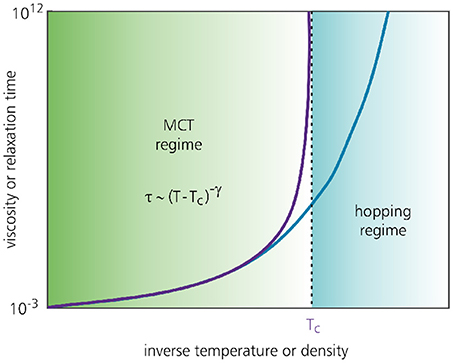
\includegraphics[width=0.65\textwidth]{hopping-region.jpg}
    \caption{Hopping mechanism restores ergodicity. From Figure~8 in \cite{mct-primer}.}
\end{figure}

\section{Connection with other systems}

It can be found that the approach we derive MCT is quite straightforward and universal. We expect MCT to be 
connected with systems more than molecular glasses. Actually, schematic MCT is \emph{exact} for some spin 
glasses.

\bibliographystyle{plain}
\bibliography{glass} 

\end{document}